
  En este capítulo se describe el diseño del lenguaje \frob{} junto con su semántica.
  Luego se explica de qué manera es traducido al lenguaje \alf{} de bajo nivel, mas
simple de interpretar, el cual podrá ser interpretado por implementaciones de
una máquina virtual en diferentes plataformas de hardware.

  También se describirán las etapas de compilación, desde que se escribe
un programa en alto nivel hasta que el mismo es ejecutado en una
plataforma objetivo.

  El diagrama de la Figura \ref{fig:compilacion} resume todas las etapas y
componentes necesarios:

\begin{figure}[h]
\begin{center}
\caption{Etapas y componentes}
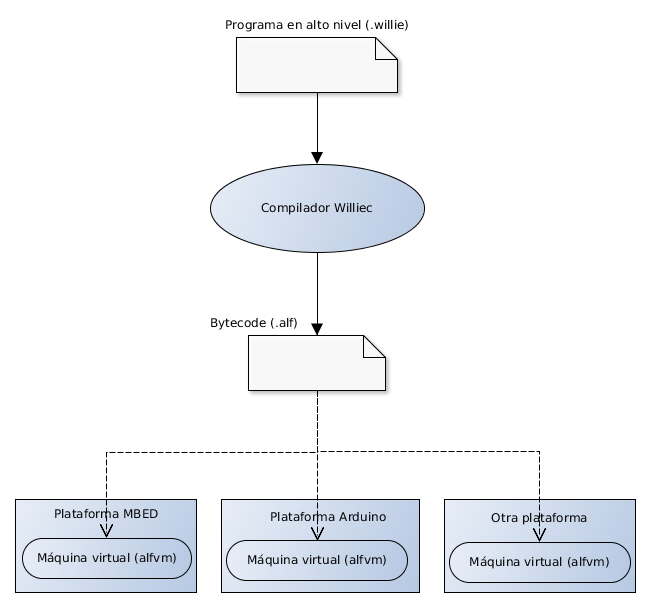
\includegraphics[width=0.9\textwidth]{graphs/compilacion.png}
\label{fig:compilacion}
\end{center}
\end{figure}

  El desarrollador escribirá su programa en el lenguaje \frob{} de alto
nivel, ejecutará el compilador y obtendrá un archivo \alf{} binario.

  Por otro lado el robot objetivo, tendrá instalada la máquina
virtual (alfvm) correspondiente a la plataforma del mismo.

  El desarrollador podrá enviar su código \alf{} al robot, y la máquina
virtual se encargará de interpretarlo.

